%!TEX root = ../main_article.tex

\section{Methodology}

We propose two strategies to improve code search performance based on the assumption that identity information will confuse the model when fine-tuning multiple language data. Instead of changing the structure and pre-training the whole code search model, we focus on transforming the model output embedding vectors during the fine-tuning process, which is less computing complexity. 

The first strategy is leveraging GAN to eliminate identity information. The second strategy is to distance the KL divergence (CITE) between identity embedding and semantic embedding.

\noindent\textbf{Identity and semantic information.} The identity information we consider as the syntax signal of different program languages, which distinguishes them from each other. We consider the identity information as the signal that the model can classify each program language data correctly. The semantic information is the intention of a code snippet, which describes the function of the code.

\subsection{Strategy 1}

In this section, we introduce a GAN-based enhance network, 
which contains a generator and a discriminator. 
We start by introducing the basic idea and the model structure. 
Then we describe the training procedure in this paper in detail. 

\begin{figure}[htb]
	\centering
	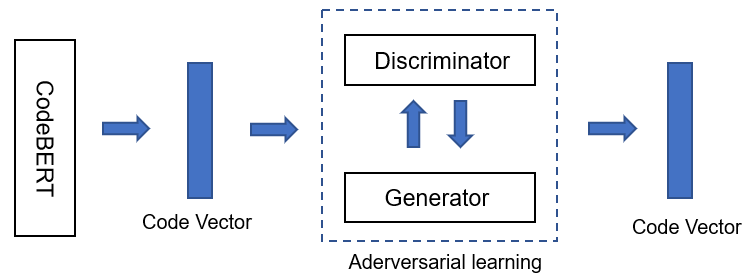
\includegraphics[width=1\linewidth]{imgs/structure.png}
	% \vspace{-15pt}
	\caption{Structure of the search enhancement framework.}
	% \vspace{-12pt}
	\label{fig:structure}
\end{figure}

The GAN structure is used widely in image generation. 
Generally, it contains two sub-network: a generator, 
which aims at generating data of a specific distribution, and a discriminator, 
which intends to determine the generated data if it is in the ideal distribution. 
In this paper, we introduce an MLP (Multilayer Perceptron) as the generator, 
of which the purpose is to generate high-dimensional vectors free of identity information. 
We also use another MLP as the discriminator. 
The object of the discriminator is to determine whether the vector generator produced 
contains identity information. The structure of the network can be seen in Fig~\ref{fig:structure}.

\begin{figure}[htb]
	\centering
	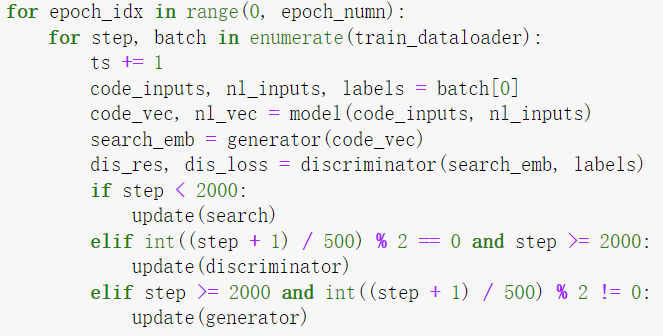
\includegraphics[width=1\linewidth]{imgs/gan_torch.png}
	% \vspace{-15pt}
	\caption{Pytorch style pseudocode of strategy 1}
	% \vspace{-12pt}
	\label{fig:gan}
\end{figure}

\subsection{Strategy 2}
Although GAN has a strong ability of learning and manipulating data distribution, 
it is hard to be trained, and can easily suffer from gradient vanishing (CITE). 
Therefore, we propose an MLP-based network to disentangle identity and semantic 
information. The overlook of the network can be seen in Fig~\ref{fig:st2}. 

The network takes embedding vectors extracted by CodeBERT as the input. 
Then, the input vector will be put into MLPs and can obtain 
two high-dimensional vectors: $V_1$ and $V_2$. 
We hope that $V_1$ possesses identity information and $V_2$  
possesses semantic information. Therefore, 
we use $V_1$ for classification and $V_2$ for code search, 
in order to extract identity and semantic information, respectively. 
Then, we maximize KL divergence, which is illustrated in Eq, between $V_1$ and $V_2$. 
Finally, $V_2$ can be viewed as the sentence embedding 
of a input code snippet without identity information and can be further 
used for code search.

\begin{figure}[htb]
	\centering
	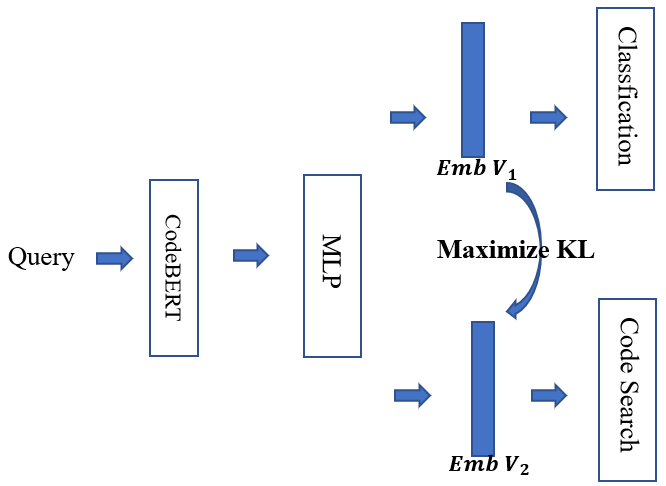
\includegraphics[width=0.8\linewidth]{imgs/st2.png}
	% \vspace{-15pt}
	\caption{Overlook of strategy 2}
	% \vspace{-12pt}
	\label{fig:st2}
\end{figure}

According to the above, learning the disentangle network 
involves finding parameters $\theta=(W,b)$ that minimize the hybrid loss on the given dataset, 
and the objective is given as Eq~\ref{eq_st2_4}, 
where $\alpha_1$, $\alpha_2$, $\alpha_3$ are hyperparameters, 
and the sum of them is equal to 1. 
Besides, Eq~\ref{eq_st2_1} represents the code search loss, intends to keep search performance, 
where $sim$ is  the similarity score and $c_i$ is the $i_{th}$ code and $q_i$  is the $i_{th}$ query. 
Eq~\ref{eq_st2_2} is the classification loss, the purpose is to extract identity information. 
Eq~\ref{eq_st2_3} leverages KL divergence to maximize the distribution of the embedding vectors output 
by the disentangle network.
\begin{equation}\label{eq_st2_1}
L_{1} = \frac{1}{n}{\sum_{i = 1}^{n}\left( 1 - sim\left( encoder\left( c_{i} \right),encoder\left( q_{i} \right) \right) \right.}
\end{equation}

\begin{equation}\label{eq_st2_2}
L_{2} = \frac{1}{n}{\sum_{i = 1}^{n}{\sum_{j = 1}^{k}{- y_{i,j}log\left( p_{i,j} \right)}}}
\end{equation}

\begin{equation}\label{eq_st2_3}
L_{3} = \frac{1}{n}{\sum_{i = 1}^{n}\left( \alpha - KL\left( V_{1,i},V_{2,i} \right) \right)}
\end{equation}

\begin{equation}\label{eq_st2_4}
\theta = {\min\limits_{\theta}{\alpha_{1}L_{1} +}}\alpha_{2}L_{2} + \alpha_{3}L_{3}
\end{equation}

